\documentclass{frontiersSCNS}

\usepackage{url,hyperref,lineno,microtype}
\usepackage[onehalfspacing]{setspace}
\linenumbers

%\usepackage[margin=1in,footskip=0.25in]{geometry}

%\usepackage{helvet}
%\renewcommand{\familydefault}{\sfdefault}

\renewcommand\refname{\vskip -1cm}


%\renewcommand{\rmdefault}{phv} % Arial
%\renewcommand{\sfdefault}{phv} % Arial
\usepackage{setspace}
\usepackage{wrapfig}
\usepackage{amsmath}
\usepackage{amssymb}
\usepackage{graphicx}
\usepackage{mathrsfs}
\usepackage{bm}
\usepackage{wasysym}
\usepackage{placeins}
\usepackage{multirow}
\usepackage[T1]{fontenc}
%\usepackage[super]{natbib}
\usepackage{framed}
\usepackage{caption}
\usepackage{longtable}


\def\keyFont{\fontsize{8}{11}\helveticabold }
\def\firstAuthorLast{Yeakel {et~al.}} %use et al only if is more than 1 author
\def\Authors{
Justin D. Yeakel\,$^{1,2,\dagger,*}$,
Uttam Bhat\,$^{1,3,\dagger}$,
Emma E. Smith\,$^3$,
and Seth D. Newsome\,$^3$}
% Affiliations should be keyed to the author's name with superscript numbers and be listed as follows: Laboratory, Institute, Department, Organization, City, State abbreviation (USA, Canada, Australia), and Country (without detailed address information such as city zip codes or street names).
% If one of the authors has a change of address, list the new address below the correspondence details using a superscript symbol and use the same symbol to indicate the author in the author list.
\def\Address{$^{1}$Santa Fe Institute, Santa Fe, New Mexico, USA \\
$^{2}$School of Natural Sciences, University of California, Merced, Merced, California, USA \\
$^{3}$Department of Physics, Boston University, Boston, Massachusetts 02215, USA \\
$^{4}$Department of Biological Sciences, University of New Mexico, Albuquerque, New Mexico, USA \\
$^{\dagger}$Contributed equally}
% The Corresponding Author should be marked with an asterisk
% Provide the exact contact address (this time including street name and city zip code) and email of the corresponding author
\def\corrAuthor{Justin D. Yeakel}
\def\corrAddress{Santa Fe Instite, Santa Fe, New Mexico, 87505, USA}
\def\corrEmail{jdyeakel@gmail.com}


\begin{document}
\onecolumn
\firstpage{1}

\title[Exploring the isotopic niche]{Exploring the isotopic niche: isotopic variance, physiological incorporation, and the temporal dynamics of foraging}

\author[\firstAuthorLast ]{\Authors} %This field will be automatically populated
\address{} %This field will be automatically populated
\correspondance{} %This field will be automatically populated

\extraAuth{}% If there are more than 1 corresponding author, comment this line and uncomment the next one.
%\extraAuth{corresponding Author2 \\ Laboratory X2, Institute X2, Department X2, Organization X2, Street X2, City X2 , State XX2 (only USA, Canada and Australia), Zip Code2, X2 Country X2, email2@uni2.edu}


\maketitle


% \begin{document}
%
% \title{Isotopic incorporation and the temporal dynamics of foraging among individuals and within populations}
% \author{JD Yeakel, U Bhatt, SD Newsome}
% \maketitle

\begin{abstract}

%%% Leave the Abstract empty if your article falls under any of the following categories: Editorial Book Review, Commentary, Field Grand Challenge, Opinion or specialty Grand Challenge.
\section{}
%As a primary goal, the abstract should render the general significance and conceptual advance of the work clearly accessible to a broad readership. References should not be cited in the abstract.
For full guidelines regarding your manuscript please refer to \href{http://www.frontiersin.org/about/AuthorGuidelines}{Author Guidelines} \\ or \textbf{Table \ref{Tab:01}} for a summary according to article type.


\tiny
 \keyFont{ \section{Keywords:} Text Text Text Text Text Text Text Text } %All article types: you may provide up to 8 keywords; at least 5 are mandatory.
\end{abstract}


\section{Introduction}

Consumer foraging behaviors are dynamic, resulting in diets that change over time as a function of environmental conditions, the densities of consumer and resource populations, and even the physiological states of individual foragers.
Understanding how diets change, and to what extent different conditions promote or inhibit specific changes, is both a challenging theoretical and empirical problem in ecology.

Analysis of carbon and nitrogen stable isotopes of a consumer with respect to a suite of potential prey is a commonly used tool for determining diet.
As a consumer incorporates the isotopic values of its consumed resources into its tissues, it becomes a unique `blend' of its prey.
Determining the most likely proportional contribution of prey that determines a given consumer's diet has thus been the focus of intense interest (REFS).

Of additional interest are the factors that control the consumer's isotopic niche width, which is defined by the isotopic variance of the consumer at either the individual or population level.
A consumer's isotopic niche width, by definition, is a function of the isotopic values of its potential prey (the prey mixing space), as well as its dietary predilections.
For a given mixing space, a consumer with a large isotopic niche width may be incorporating many isotopically distinct prey into its diet, while a consumer with a small isotopic niche width may be specializing on a single resource.


%Difference between the isotopic diet view vs. other diet views

%Backward integrating vs. Forward integrating

%EXPLORE VARIANCE ~ what controls the isotopic niche?

%Prey-switching dynamic
%Micro time frame
%Macro time frame




\section{Methods \& Analysis}
We begin by establishing a forward-integration approach for modeling the incorporation of stable isotopes from multiple resources into a consumer's tissues.
This new methodology provides an analytical link between the mechanistic drivers of foraging and the distribution of stable isotope values describing a consumer's tissues over time.
%This framework aims to provide a flexible platform for introducing additional ecological complexities, such as time-dependent foraging behaviors and dietary specialization both among and within individuals.
Using this framework, we aim to
1) examine how certain dietary behaviors, such as prey specialization and different modes of dietary variation, impact the isotopic variance of consumer tissues thus aiding ecological interpretation of the `isotopic niche', and
2) show how these methods can be expanded to include foraging behaviors that themselves are temporally dynamic, changing over seasons or years.

\subsection*{Deriving the within-individual isotopic niche width}
%The dynamics of diet ~ heuristic description of the process
There are many ways to statistically summarize the integration of prey by a consumer species, however in order to establish a mechanistic link between foraging and the consumer's isotopic composition, we follow the proceeding heuristic foraging mechanic.

We assume that a consumer encounters and consumes resources in proportion to the encounter rate of each prey; prey that are encountered more frequently are assumed to be consumed more frequently.
An alternative approach could incorporate preferences (REFS) or even state-dependence (REFS), and we will briefly address these considerations in the Discussion.
As prey are encountered and consumed, the prey's isotope values are incorporated into the consumer's tissues weighted by the prey-specific proportional contribution to diet.
The resulting distribution that descibes the dietary input of multiple prey (each with an independent Gaussian density that describes the distribution of their isotopic values) is a mixed Gaussian distribution with weights determined by the prey's proportional contribution to diet.
This proportional contribution is itself a random variable drawn from a Dirichlet density (a multivariate Beta distribution) that serves as a probabilistic description of the consumer's dietary input.
The following section details our probabilistic determination of the consumer's isotopic composition.
We focus our attention on the variability of the consumer isotopic distribution, which is equivalent to its isotopic niche width - a statistic of certain interest to ecologists using stable isotopes as a tool to understand diet.
%, as well as an analysis of the properties of the final consumer isotopic distribution.


%Derivation of the Dirichlet controlling diet
%If we  that the proportional contribution of prey to a consumer's diet scales to the rate at which it encounters its prey.
%, such that we must first describe how the Dirichlet distribution describing consumer diet at a given point in time changes as a function of prey densities.
A consumer encounters each prey at a frequency determined by a Poisson process with parameter $\psi_i$, which determines the number of encounters $M_i(t)=m_i$ between time 0 and time $t$,

\begin{equation}
f_M (m_i|\psi_i) = {\rm e}^{-\psi_i t}\frac{(\psi_i t)^m_i}{m_i!}.
\end{equation}

\noindent Here and henceforth, we use the general function $f(\cdot)$ to denote different frequency distributions, as well as uppercase notation to describe stochastic variables, and lowercase notation to describe specific values of stochastic variables.
If we assume that encounter rates are variable, such that some prey are more patchily distributed than others, we can treat $\Psi_i = \psi_i$ as a random variable with a Gamma density

\begin{equation}
f_\Psi (\psi_i | c, a_i) = \frac{c^{a_i}}{\Gamma (a_i)}{\rm e}^{-c \psi_i}\psi_i^{a_i - 1}.
\end{equation}

\noindent Here, $a_i$ is the dispersion parameter, which is proportional to the encounter rate, and $c$ scales with the time between encounters.
If we integrate across all possible values of $\psi_i$, we obtain the Negative Binomial density with mean encounter rate $a_i/c$ and coefficient of variation $1/\sqrt{a_i}$ (REF Mangel).
Following the derivation described by Ainsworth (REF), if we define the proportional contribution of prey to a consumer's diet to scale with the encounter rate, such that

\begin{equation}
  p_i = \frac{\psi_i}{\sum_{j=1}^n \psi_j},
\end{equation}

\noindent then the random variable $P_i \in {\bm P} = p_i \in {\bm p}$, where $\sum_i p_i = 1$, has a Dirichlet distribution with density

\begin{equation}
  f_{\bm P}(p_1,...,p_n|a_1,...,a_n) = \frac{\Gamma(\sum_{i=1}^n a_i)}{\sum_{i=1}^n\Gamma(a_i)}\prod_{i=1}^n p_i^{a_i - 1},
\end{equation}

\noindent where $\Gamma(\cdot)$ is the gamma function (REF Mangel).
We note that bold-face fonts denote vectors of variables.
As such, the expected proportional contribution of a prey $i$ to the consumer's diet has the expectation ${\rm E}\{p_i\}=a_i/a_0$ where $a_0 = \sum_i a_i$, and variance

\begin{equation}
  \label{eqDirVar}
  {\rm Var}\{p_i\} = \frac{a_i(a_0 - a_i)}{a_0^2(a_0 + 1)}.
\end{equation}

\noindent Accordingly, we assume each time interval represents a single foraging bout, where we draw a single prey $i$ with probability $p_i$ for inclusion to the consumer's diet.

Describing the dietary behavior of a consumer as a Dirichlet distribution provides a flexible and powerful framework to investigate how different foraging strategies influence a consumer's isotopic niche.
For example, a pure generalist consumer would have a Dirchlet distribution with parameters $a_i = 1$ for all prey $i=1,...,n$, such that the marginal distribution for $P_i = p_i$ is close to uniform with expectation ${\rm E}\{p_i\} = 1/n$.
Because we have assumed that the proportional contribution of a prey to the consumer's diet scales with the prey's encounter rate, this would be analogous to a system where a consumer is equally likely to encounter the same number of any prey.
In contrast, an obligate specialist would have a Dirichlet density that is spiked for a given prey $k$, such that the single parameter $a_k \gg 1$, while $a_{i \neq k} = 1$.
The use of a Dirichlet distribution is also at the heart of Bayesian isotope mixing models (REFS), which assume a Dirichlet prior and enable the input of alternative dietary information to inform isotopic data.



%Describing Z
If the isotopic distributions for the set of potential prey follow independent Gaussian distributions, and the dietary behavior of the consumer has a Dirichlet density, the resultant density that describes the isotopic distribution of a consumer's diet $f_Z(Z=z)$ is a mixed Gaussian distribution, with weights given by $\bm p$ drawn from the Dirichlet distribution.
This density can be written as

\begin{equation}
  \label{eqfZ}
f_Z(z|{\bm p},{\bm \mu},{\bm \sigma}) = \sum_{i=1}^n p_i\frac{1}{\sqrt{2 \pi \sigma_i^2}}{\rm e}^{-\frac{(z-\mu_i)^2}{2\sigma_i^2}},
\end{equation}

\noindent with the expectation

\begin{equation}
\label{eqEZ}
  {\rm E}\{Z\} = \sum_{i=1}^n \frac{a_i}{a_0} \mu_i,
\end{equation}

\noindent where $\mu_i$ is the mean isotopic value for prey $i$.
This is simply the weighted average of the isotopic values for the prey community, where weights are determined by the mean proportional contribution of prey to the consumer's diet.

Of more interest to us here is the variance of $Z$, which will allow us to analytically determine the isotopic niche width of the consumer as a function of its dietary behavior and the isotopic distributions (or mixing space) of its prey.
We find that

\begin{equation}
\label{eqVarZ}
  {\rm Var}\{Z\} = \sum_{i=1}^n \frac{a_i}{a_0}\left(\sigma_i^2 + \mu_i^2\right) - \frac{a_i^2\mu_i^2}{a_0^2}-\sum_{i \neq j}\frac{a_i a_j \mu_i \mu_j}{a_0^2}.
\end{equation}

\noindent Although the form of Eq. \ref{eqVarZ} is not intuitive, we emphasize that - over different dietary behaviors that shape the Dirichlet distribution and for different isotopic mixing spaces - it is this equation that governs the expansion or contraction of the consumer's isotopic niche width, and therefore of chief ecological interest.

The isotopic variance of the consumer's diet ${\rm Var}\{Z\}$ can be simplified by considering a specific set of dietary behaviors.
Here we examine how ${\rm Var}\{Z\}$ is influenced by generalist vs. specialist consumer diets, as well as the role of general mixing space geometries, in determining consumer isotopic niche width.
If a generalist consumer alters its diet to include more of a certain prey $k$ relative to the others, the Dirichlet distribution that defines its dietary behavior goes from $a_i=1$ for all $i=1,...,n$ to $a_{i \neq k}=1$ for $i=1,...,n$, with $a_k>1$.
As specialization increases, the Dirichlet parameter corresponding to the targeted prey $k$, increases to a value much higher than one (pure specialization is obtained only at the limit $a_k \to \infty$).
Thus, we can assume that $a_i=1$ for all $i \neq k$, and $a_k = (n-1)s_k/(1-s_k)$, where $s_k$ denotes specialization on prey $k$, ranging from $1/n$ (generalization) to $1$ (specialization).
We can thus substitute $a_0 = (n-1)/(1-s_k)$ and $p_i = a_i/a_0 = (1-s_k)/(n-1)$ for all $i \neq k$, and $a_k/a_0 = s_k$.
We can then rewrite Eq. \ref{eqVarZ} as

\begin{equation}
\label{eqVarZs}
{\rm Var}\{Z\} = \frac{1-s_k}{n-1}\sum_{i \neq k}^n \left(\sigma_i^2 + \mu_i^2\right) + s_k(\sigma_k^2 + \mu_k^2) - \left(\frac{1-s_k}{n-1}\sum_{i \neq k}^n \mu_i + s_k\mu_k \right)^2,
\end{equation}

\noindent and note that, independent of the prey mixing space (a function of $\mu_i$ and $\sigma_i^2$ for prey $i=1,...,n$), the isotopic variance of the consumer's diet will always be a concave parabolic function over $s_k$.
With respect to the size of the consumer's isotopic niche width, this means that there can be a peak variance for a value of $s_k$ intermediate to pure generalization ($s_k=1/n$) and pure specialization ($s_k=1$).

The peak $\hat s_k$, that describes the maximum isotopic variance of the consumer may or may not fall between $s_k=1/n$ and $s=1$, and is only of ecological interest if it does.
The peak variance can be solved analytically by setting the derivative of Eq. \ref{eqVarZs} with respect to $s_k$ equal to zero, and solving for $s_k$, which results in

\begin{equation}
	\hat s_k = \frac{A(1-n)+B (n-1)^2+2 C (C-D n+D)}{2 (C-D n+D)^2},
\end{equation}

\noindent where $A = \sum_{i \neq k}^n \left(\sigma_i^2 + \mu_i^2\right)$, $B = \left(\sigma_k^2 + \mu_k^2\right)$, $C = \sum_{i \neq k}^n \mu_i$, and $D = \mu_k$.

Determination of the peak variance allows us to predict where the consumer's isotopic niche is expected to be maximized as a function of specialization on different prey.
Although here we have focused on the special case where a consumer targets a single prey, one can rewrite the equation for the consumer's isotopic niche width with respect to increasing specialization on any number or combination of prey in the mixing space.
For example, in the case where a consumer specializes on two prey (i.e. two species of crab), one would rewrite Eq. \ref{eqVarZ} in terms of both $s_k$ (specialization on prey $k$) and $s_l$ (specialization on prey $l$), resulting in a concave parabolic plane in dimensions $s_k$ and $s_l$.
Determining the maximum variance would then entail taking the derivative of Eq. \ref{eqVarZ} with respect to both $s_k$ and $s_l$.
In dimensions higher than 2, the process would be the same, with the goal of finding the maximum variance over a hyperplane with a number of dimensions determined by the number of prey on which the consumer is preferentially targeting.
Because specializing on multiple prey does not introduce anything conceptually unique, we consider only the case of a single-prey specialist.



\subsection*{The Dynamics of Isotopic Incorporation}
We have established a framework for analytically calculating the distribution of isotope values that characterizes a consumer's diet, composed of multiple, isotopically distinct prey.
The dietary behavior of the consumer is a function of a single Dirichlet distribution, which is assumed not to change over time, although we will relax this assumption in the next section.
By the central limit theorem, over long timescales the dietary distribution of the consumer is static, with a fixed mean and variance.
However, over short timescales, the diet of the consumer varies as Eq. \ref{eqDirVar}, while its isotopic values vary by the combined effects of the Dirichlet and the mixed Gaussian framework, described by Eq. \ref{eqVarZ}.

%Not sure, but this might be more appropriate in the discussion
As the consumer incorporates prey into its diet, the isotopic distribution of its diet is incorporated into its tissues.
The timescale of physiological isotopic incorporation is based on the turnover rate of consumer tissues, which on the fast end can occur within days to weeks (e.g. blood plasma), and on the slow end occur over years (e.g. bone).
Incorporation rates are well known to isotope ecologists and have been observed in both controlled feeding studies (REFS), and occasionally in the wild (REFS?).
Although the physiological details are not well understood, isotopic incorporation can be modeled using either single- or multi-compartmental approaches (REFS).
In a single compartment framework, isotope ratios are ingested with food, and directly incorporated into consumer tissues at a tissue-specific rate.
In multiple compartment frameworks, it is assumed that incorporation occurs over multiple body pools, the turnover of each occuring at different rates.
Though an assumption of multi-compartmental incorporation often does provide better statistical fit with experimental data (REFS), the physiological processes that drive incorporation of isotope ratios from one compartment to the other are not well understood (REF), and such fits are only marginally better than a single-compartment approach.

In this next section, we assume that the ingested isotope ratios are incorporated into consumer body tissues directly, moderated by the rate of incorporation $\lambda$, which is treated as a free parameter.
For simplicity, we assume that time is scaled such that a single time step corresponds to a single foraging bout.
Moreover, we assume that the consumer is incorporating prey of smaller size than itself, such that $ 0 < \lambda < 1$.
Thus, we aim to determine the isotopic composition of the consumer $X_c$ as a function of the consumer diet, the isotopic distribution of its prey (or mixing space), and $\lambda$.
% The carbon and nitrogen isotope composition of a consumer's tissues are a product of its diet.
% If this diet incorporates multiple prey in different quantities, as is the case for most consumers, the resulting consumer isotopic distribution must take into account:
% \emph{i}) the initial isotopic signature of the consumer's tissues at a point in time $X_c(t)$ (we will assume for simplicity that the isotopic value in question is the ratio of heavy to light carbon isotope relative to a known standard $\delta^{13}{\rm C}$, though are methods are equivalent for any isotope that is integrated through diet),
% \emph{ii}) the isotopic values of $n$ resources, which we assume are Gaussian distributed with expectation $\mu_i$ and variance $\sigma_i^2$,
% %$\sum_{i=1}^n p_i \mu_i$ (where $p_i$ is the proportional contribution of resource $i$ and $\mu_i$ is the mean isotopic value of resource $i$),
% \emph{iii}) the rate at which each prey species is ingested by the consumer, summarized by its proportional contribution $p_i$,
% and
% \emph{iv}) the incorporation rate of a consumer's diet into its tissue $\lambda$.
In a completely deterministic framework, the isotopic composition of the consumer can be written as an ordinary differential equation

\begin{equation}
\label{eqODE}
\dot X_c = (1-\lambda)X_c + \lambda \sum_{i=1}^N p_i \mu_i - X_c
\end{equation}

\noindent where the overdot denotes the derivative with respect to time $t$, and $p_i$ and $\mu_i$ are the proportional contribution of prey $i$ to the diet of the consumer, and the mean isotopic value of prey $i$, respectively.

However, we must also take into account the stochastic effects described in the previous section, inluding the variation associated with the consumer's diet, as well as the isotopic variation of each potential prey.
% First, each potential resource $i$ is composed of individuals with isotopic values varying according to independent Gaussian distributions with expecation ${\rm E}\{X_i\}=\mu_i$, and variance ${\rm Var}\{X_i\}=\sigma^2_i$.
% Secondly, in this section we consider a consumer diet is variable, yet static (such that it can be described by a time-invariant probability distribution), there is variation in the consumption of prey across short periods of time.
We account for these stochastic effects by describing changes in the consumer's isotopic distribution with the stochastic differential equation

\begin{equation}
\label{eqSDE}
{\rm d}X_c = (1-\lambda)X_c{\rm dt} + \lambda\left({\rm E}\{Z\}{\rm dt} + \sqrt{{\rm Var}\{Z\}}{\rm dW}\right) - X_c{\rm dt}.
\end{equation}

\noindent where ${\rm dW}$ is the increment of Brownian motion (REF MANGEL).
This stochastic differential equation describes a process known as an Orstein-Uhlenbeck process, which describes a stochastic process that has a steady state variance around the mean.
Because the time interval ${\rm dt}$ is infinitely short at the continuous limit, the consumer's isotopic distribution will have a Gaussian density (REF).
In this case, if the initial isotopic values of the consumer at time $t=0$ is $X_c(0)$, the expectation and variability of $X_c$ at time $t$ are

\begin{align}
  \begin{split}
    \label{eqEVar}
{\rm E}\{X_c(t)\} &= {\rm E}\{Z\} + (X_c(0) - {\rm E}\{Z\}){\rm e}^{-\lambda t},\\
{\rm Var}\{X_c(t)\} &= \frac{\lambda {\rm Var}\{Z\}}{2}\left(1 - {\rm e}^{-2\lambda t}\right).
\end{split}
\end{align}

\noindent where ${\rm E}\{Z\}$ and ${\rm Var}\{Z\}$ are as defined in Eqns. \ref{eqEZ} and \ref{eqVarZ}.
One can observe that as $t$ increases, the exponential part of ${\rm E}\{X_c(t)\}$ and ${\rm Var}\{X_c(t)\}$ go to zero, such that ${\rm E}\{X_c(t)\} \to {\rm E}\{Z\}$, and ${\rm Var}\{X_c(t)\} \to \lambda{\rm Var}\{Z\}/2$.
In other words, the expectation of the consumer's isotopic distribution will equilibrate to that of its diet, while its variance will always be less than the variance of its diet by a factor of $\lambda/2$.
Variance decreases as the rate of incorporation decreases due to the consumer averaging its isotopic value over more prey (because the tissue is turning over more slowly), and this serves to average out fluctuations in the consumer's diet.
% This decrease in variance is due to the fact that the consumer-diet mix has a biased weight towards its own body tissues, such that $\lambda < 1(2)$.
%if \lamabda = 2, then it will look like what it eats... weird... worth going into at all?




% This is in accordance with known exponentially-decaying isotopic values of consumers shown in controlled-diet experiments (REFS).

%By uniting both dietary and isotopic variability into the single random variable $Z$, the above framework provides a means towards predicting the isotopic composition of a consumer over time, given a dietary strategy (described by the Dirichlet distribution) and the isotopic distribution of the potential resources (the isotopic mixing space).
%Permitting the consumer's dietary strategy to vary provides a direct means of incorporating behavioral variability in estimates of a consumer's isotopic composition.





%\subsection*{Temporal dietary dynamics}
An implicit assumption of the static model is that the consumer's diet varies instantaneously over a given parameterization of $f_Z(Z)$.
This is relevant for organisms that have a consistently varying diet over time, however most organisms have diets that undergo large changes over longer periods time.
In such cases, the Dirichlet distribution that characterizes diet during one small temporal interval will be different than the Dirichlet distribution characterizing diet during another interval far apart in time.
Such a shift might be due to seasonal, ontogenetic, or demographic changes in the consumer's prey base over the course of months to years.
In the following section, we will relax the assumption that diet is characterized by a single Dirichlet distribution over time, thus generalizing our formulation of consumer isotopic dynamics as a function of time.

As the consumer's diet changes over time, the random variable of interest is now $Z(t)$, which is the trajectory defining the isotopic values of the consumer's diet over time.
Solving for $X(t)$, we find

\begin{align}
  \label{eqEVarZt}
{\rm E}\{X(t)\} = X(0){\rm e}^{-\lambda t} + \lambda{\rm e}^{-\lambda t} \int_{s=0}^t {\rm e}^{\lambda s} {\rm E}\{Z(s)\}{\rm d}s, \nonumber \\
{\rm Var}\{X(t)\} = \lambda^2 {\rm e}^{-2\lambda t} \int_{s=0}^t {\rm e}^{2\lambda s} {\rm Var}\{Z(s)\} {\rm d}s.
\end{align}



% Incorporating different classes of prey-switching dynamics permits an understanding of how the isotopic composition of a consumer reflects changes in its behavior over time as a function of the incorporation rate $\lambda$.
% To gain an intuitive understanding of how ecological dynamics are portrayed by consumer isotope values, we consider two types of prey-switching behavior: {\it i}) an instantaneous shift from one dietary strategy to another (such as those used in feeding experiments), and {\it ii}) a sinusoidally varying dietary strategy.




\section{Results}

As a consumer samples from multiple prey with stable isotopes values following independent Gaussian distributions, its tissues become a mixture of these distributions.
The weights that control the contributions of each prey to the consumer mix are determined by the dietary behavior of the consumer, which we have shown follows a Dirichlet distribution.
The use of the Dirichlet distribution in this context follows previous ecological models by Ref(Ainsworth, others?), and is also used as a prior in Bayesian isotope mixing models.
We note that Bayesian mixing models are essentially models that explore the opposite question that we are investigating: they are used to estimate the dietary behavior of the consumer (the posterior probability distribution for the proportional contribution vector $\bm p$) given the isotopic distributions of both consumer and prey, whereas we are investigating factors that impact the isotopic distribution of the consumer as a function of different prey mixing spaces and consumer dietary behaviors.


We have provided an analytical solution for the mean and variance of the consumer's isotope distribution as a function of its diet and the isotope mixing space.
By formulating these solutions in terms of consumer generalization and specialization, we make three observations:
1) the variance of the consumer's isotope distribution (${\rm Var}\{Z\}$), which is equivalent to its isotopic niche width, is concave parabolic;
2) whether and to what extent the ${\rm Var}\{Z\}$ demonstrates measurable nonlinearity depends in part on the geometry of the mixing space;
3) the inversion point, or the peak, of ${\rm Var}\{Z\}$ over the generalization-specialization continuum is the consumer's maximum isotopic niche width.
This point may or may not exist at a value intermediate to an obligate generalist or obligate specialist.


%1-2: Concave parabolic variance curve & geometry of mixing space

% The width, or variance, of the consumer's isotopic niche is necessarily concave parabolic over the specialization metric $s$, where $s=1/n$ refers to an obligate generalist, and $s=1$ refers to an obligate specialist.
% This means that there is a peak isotopic variance that lies somewhere along this specialization continuum, however it is only of interest to us of it lies in $s \in [1/n,1]$.



\subsection*{Temporally variable diets}
%Incorporation results
The equilibrial solution to our stochastic differential equation (Eq. \ref{eqSDE}) reveals that the isotopic variability of the consumer scales to diet as a factor of $\lambda/2$.
As the incorporation rate decreases, such that the turnover time is long, the isotopic variability of the consumer declines.
Moreover, we observe that as the consumer transitions from some initial isotopic state $X_c(0)$ to diet, the variance of the consumer's isotopic values equilibrate twice as fast as the mean value, as shown in the exponential component of Eq. \ref{eqEVar}.

%Dynamic diet results
If the consumer's diet is itself variable over time, we do not expect its isotopic composition to equilibrate as it would in a controlled feeding study.
For example, the consumer might adopt one diet during the wet season, and another during the dry season, such that it oscillates between the two throughout the year.
We consider a composite diet with an isotopic distribution $\mathbb Z ~ f_{\mathbb Z}$ that dynamically oscillates between two subdiets, which we will refer to as `seasonal diets'.
The seasonal diets have random variables $Z_1$ and $Z_2$, distributed according to Eq. \ref{eqfZ}, where each has a different underlying Dirichlet -- encoding which prey the consumer targets during each season with frequency distributions $f_{\bm P_1}$ and $f_{\bm P_2}$ -- while the isotopic distributions of prey are assumed to be constant through time.
We can thus describe the composite diet as a mix of the seasonal diets, where the mix is characterized by weights that oscillate over time, $\mathcal{U}(t)$, and this determines the contribution of each seasonal dietary strategy to the whole.
The frequency distribution for the composite diet is thus

% \begin{equation}
%   f_{\mathbb{Z}(t)} = \left(\mathcal{U}(t) \sum_{i=1}^n p_{1,i}{\rm Gaus}_i( z | \mu_i,\sigma_i) + (1-\mathcal{U}(t)) \sum_{i=1}^n p_{2,i}{\rm Gaus}_i( z | \mu_i,\sigma_i)\right)f_{\bm P_1}f_{\bm P_2}
% \end{equation}

\begin{equation}
  f_{\mathbb{Z}(t)} = \left(\mathcal{U}(t) f_{Z_1} + (1-\mathcal{U}(t)) f_{Z_2}\right)f_{\bm P_1}f_{\bm P_2}.
\end{equation}

% \noindent where $\rm Gauss_i( z | \mu_i,\sigma_i)$ is the Gaussian distribution describing the isotope values for prey $i$, while $f_{\bm P_1}$ and $f_{\bm P_2}$ are the Dirichlet distributions for subdiets 1 and 2, respectively.
% \noindent where $f_{Z_1}$ and $f_{Z_2}$ are independent mixed distributions as defined in Eq. \ref{eqfZ} for diets 1 and 2, while $f_{\bm P_1}$ and $f_{\bm P_2}$ are the Dirichlet distributions for subdiets 1 and 2, respectively.

If we do not specify the type of oscillation that drives changes in diet over time, the expectation and variance for the isotopic distribution of the composite diet over time are

\begin{align}
  \label{eqZtgen}
  \begin{split}
    {\rm E}\{\mathbb{Z}(t)\} &= \mathcal{U}(t){\rm E}\{Z_1\} + (1-\mathcal{U}(t)){\rm E}\{Z_2\}, \\
    {\rm Var}\{\mathbb{Z}(t)\} &= \mathcal{U}(t){\rm Var}\{Z_1\} + (1-\mathcal{U}(t)){\rm Var}\{Z_2\} + \mathcal{U}(t)(1-\mathcal{U}(t))\left({\rm E}\{Z_1\} - {\rm E}\{Z_2\}\right)^2,
  \end{split}
\end{align}

\noindent where the mean isotopic value of the composite diet is averaged over both seasonal diets, weighted by the proportional inclusion of each.
In the wet/dry season example, the consumer could either shift gradually from its wet season diet to its dry season diet if $\mathcal{U}(t)$ is smooth, or shift abruptly if $\mathcal{U}(t)$ is a step function.
An example of the latter scenario would be a grizzly bear consumer system, where its diet shift abruptly with the arrival of salmon during spawning season (REF).


Most dietary transitions between seasons tend to be gradual, even if the end/start of a given season is abrupt (REF).
To understand how a temporally oscillating diet affects the isotopic variance of the composite diet, we consider the smooth oscillation $\mathcal{U}(t) = 1/2 + 1/2\sin(\omega t)$, which determines the proporitonal contribution of diet 1.
Here, $\mathcal{U}(t)$ varies between 0 and 1, with a frequency $\omega$ (Fig. \ref{figvarZt}A).
Substituting $\mathcal{U}(t)$ into Eq. \ref{eqZtgen} provides the solution to a sinusoidally varying diet, where

\begin{align}
  \begin{split}
  \label{eqZtsin}
    {\rm Var}\{\mathbb{Z}(t)\} = &\overbrace{\frac{{\rm Var}\{Z_1\} + {\rm Var}\{Z_2\}}{2} + \frac{1}{2} \left(\frac{{\rm E}\{Z_1\} - {\rm E}\{Z_2\}}{2}\right)^2}^{\alpha_{\rm V}} \\
    &+ \overbrace{\frac{{\rm Var}\{Z_1\} - {\rm Var}\{Z_2\}}{2}}^{\beta_{\rm V}}\sin(\omega t) + \overbrace{\frac{1}{2}\left(\frac{{\rm E}\{Z_1\} - {\rm E}\{Z_2\}}{2}\right)^2}^{\gamma_{\rm V}}\sin\left(2\omega t + \frac{\pi}{2}\right).
  \end{split}
\end{align}

\noindent where we have combined the non-oscillating components into three parameters $\alpha_{\rm V}$, $\beta_{\rm V}$, and $\gamma_{\rm V}$ for notational efficiency.

We gain two key insights from the solution for the variance of the composite diet.
1) The time-averaged variance (denoted by $\langle \cdot
\rangle_t$) is simply $\langle {\rm Var}\{\mathbb{Z}(t)\} \rangle_t = \alpha_{\rm V}$, which is only impacted by the average variance between the seasonal diets and the difference in the mean isotope values between the seasonal diets (Fig. \ref{figvarcont}), and
2) the oscillating component shows that the composite dietary variance has twice the frequency of the diet shift $\mathcal{U}(t)$, as well as a $\pi/2$ offset, meaning that the maximal variance of the consumer's composite diet will occur during the transition from one diet to the other (Fig. \ref{figvarZt}B).
Together, these results reveal that if the consumer's diet is varying continuously over time between two seasonal diets, both the mean variance, as well as the difference in the mean isotope values of the seasonal diets -- directly reflecting the heterogeneity of prey mixing space geometry -- will serve to increase the time-averaged variance of the consumer's diet, and by extention the isotopic variance of the consumer itself.

Less intuitively, we observe that the consumer's peak variance, or niche width, as measured by the variance of its composite diet, occurs not during the exclusive adoption of its wet/dry season diets, but during the transition between the two, and this peak variance is driven exclusively by the difference in means between seasonal diets.
As the seasonal diets become more heterogeneous in isotopic space, the greater the consumer's peak variance during the transtion, and this occurs because it is sampling between two dietary strategies that are isotopically distinct.
We can directly observe this by considering a transition between two diets with  a) different means and the same variances, and b) the same means and different variances.
In the former case, the peak variance of the composite diet occurs during the transition (Fig \ref{figvarZt}B); in the latter case, because the diets have the same mean isotope value, the peak occurs not during the transition, but when the consumer adopts the diet with the greater variance, which in our example would occur at the height of the season (Fig \ref{figvarZt}C).

%Consumer diet X_c(t)
The isotopic composition of a consumer $X_c(t)$ during a single dietary shift is governed by a single timescale of physiological origin: the rate of incorporation $\lambda$.
However, a seasonally shifting diet that is driven by oscillating foraging strategies introduces an additional ecological timescale that will affect $X_c(t)$, determined by the frequency of diet switching $\omega$.
Depending on the turnover rate of the tissue of interest and how often the consumer shifts its diet, the ratio of these timescales $\omega/\lambda$ will impact how the isotopic mean and variance of the consumer changes over time.
For the case of sinusoidally varying diet, we can solve for $X_c(t)$ directly, such that

\begin{align}
  \label{eqXsin}
  \begin{split}
    {\rm Var}\{X_c(t \to \infty)\} = &\alpha_{\rm V}\frac{\lambda}{2} + \beta_{\rm V}\frac{\lambda^2}{\sqrt{(2\lambda)^2 + \omega^2}}\sin\left(\omega t -\theta_1\right) \\
    &+ \gamma_{\rm V}\frac{\lambda^2}{2\sqrt{\lambda^2 + \omega^2}}\sin\left(2\omega t + \theta_2\right).
  \end{split}
\end{align}

\noindent where the offsets $\theta_1$ and $\theta_2$ are $ \tan^{-1}(\omega/2\lambda)$ and $ \tan^{-1}(\lambda/\omega)$, respectively.
As in the static case (where diet was not varying over long periods of time), the time-averaged variance is $\alpha_{\rm V}\lambda/2$.
Moreover, we observed that the consumer's isotope composition lags behind changes in diet, such that an isotopic shift in the consumer's tissues is observed after the actual foraging shift.
This lag involves both $\theta_1$ and $\theta_2$, however these offsets play different roles in contributing to the lag for different mixing space geometries.
When the isotopic means of the seasonal diets are similar, the lag is mostly due to $\theta_1$; when the means are different and the variances are similar, the lag is mostly due to $\theta_2$; when both the isotopic means and variances of the seasonal diets are different, both contribute significantly to the lag.
%We can quantify the timing of this shift from Eq. \ref{eqXsin}, and observe that it is XXXX.


Increasing $\omega/\lambda$, such that the timescale of ecological switching relative to that of isotopic incorporation decreases, we observe that
%we observe that as the frequency of the dietary shift increases relative to the rate of incorporation,
1) the lag between the transition and the peak variance of the consumer increases with decreasing $\lambda$, and
2) the amplitude of the variance of $X_c(t)$ decreases with increasing $\omega$.
The first result is not surprising, as it mirrors the role of $\lambda$ in the static diet example. %when diet did not change over long periods of time.
The second result is less intuitive: in words, as the consumer shifts its diet more frequently, there is still a peak variance during dietary transitions, though with diminishing amplitude, and this would make it more difficult to measure.
This is due to the consumer slowly integrating isotope ratios from both diets, thus averaging across diet-switching events.
Accordingly, the decrease in the amplitude of isotopic variance of the consumer's tissue is an averaging effect, where the timescale of incorporation is much larger than the timescale of dietary switching.
%Accordingly, we observe that as a consumer adopts a more frequently shifting diet, changes in its variance will become more damped and difficult to measure, while as the rate of incorporation decreases, the lag between shifts in diet and the isotopic value of the consumer will increase.




% However, if the consumer's diet is itself variable, we do not expect the isotopic distribution of the consumer to equilibrate as it would in a controlled feeding study.
% A common example of such a temporally dynamic diet is one that varies from one season to another; for example, we might assume that if the consumer exhibits one dietary strategy in the dry season, and another in the wet season, the expectation of the proportional contribution of prey to the consumer's diet would oscillate sinusoidally.
%
% The isotopic distribution of a consumer over time $X_c(t)$ during a single dietary shift (as in a controlled feeding study) is governed by a single physiological timescale: that of the rate of incorporation.
% In contrast, a sinusoidal dietary dynamic introduces a timescale that affects the isotopic composition of the consumer of ecological origin.
% To illustrate this interplay of both physiological and ecological timescales on how a consumer's isotope composition changes over time, we consider a diet with an isotopic mean and variance that changes sinusoidally over time, such that
%
% \begin{align}
%   \begin{split}
%     \label{eqSinZ}
%     {\rm E}\{Z(t)\} &= \alpha_{\rm E} + \beta_{\rm E}\sin(\omega t), \\
%     {\rm Var}\{Z(t)\} &= \alpha_{\rm V} + \beta_{\rm V}\sin(\omega t)
%   \end{split}
% \end{align}
%
% \noindent Here, $\alpha_{\rm E}$ is the central tendency of the oscillating mean dietary isotope values, while $\beta_{\rm E}$ is the amplitude of the mean dietary isotope values.
% Because we are simulating a continuous switch between two dietry strategies, $\beta_{\rm E}$ effectively measures the difference in the mean isotope values for each strategy.
% Because we do not assume that both dietary strategies have the same variance, we have a similar equation for ${\rm Var}\{Z\}$, where $\alpha_{\rm V}$ is the mean isotopic variance between each dietary strategy, and $\beta_{\rm V}$ determines the amplitude of the variance.
% As the difference in the isotopic variance of each dietary strategy increases (e.g. a low isotopic variance for the dry season diet, and a high isotopic variance for the wet season diet), $\beta_{\rm V}$ increases.
% Both the mean and the variance share the frequency $\omega$, and it is this term that determines the ecological timescale of the consumer's isotopic composition; a high frequency implies a greater number of shifts between dietary strategies over a given amount of time, while a low frequency implies fewer shifts.
%
% To determine the effect of an oscillating diet on the consumer's isotope distribution, we must solve Eq. \ref{eqEVarZt}, where ${\rm E}\{Z(t)\}$ and ${\rm Var}\{Z(t)\}$ are as defined in Eq. \ref{eqSinZ}.
% Doing this and throwing out the exponentially decaying components of the equation (which describes the transition to the shifting diet from some intitial condition $X_c(0)$, we find that the isotopic mean and variance of the consumer is written
%
% \begin{equation}
% \label{EX-sin}
% {\rm E}\{X_c\} = \alpha_{\rm E} + \frac{\beta_{\rm E} \lambda}{\sqrt{\lambda^2+\omega^2}} \sin{\left(\omega t - \tan^{-1}{\left(\frac{\omega}{\lambda}\right)}\right)}
% \end{equation}
% \begin{align}
% \label{VX-sin}
% {\rm Var}\{X_c\} = \frac{1}{4}\lambda\left(2 \alpha_{\rm V}^2 + \beta_{\rm V}^2\right) &+ \frac{2 \alpha_{\rm V} \beta_{\rm V} \lambda^2}{\sqrt{4\lambda^2+\omega^2}} \sin{\left(\omega t - \tan^{-1}{\left(\frac{\omega}{2\lambda}\right)}\right)} \nonumber \\ &- \frac{\beta_{\rm V}^2\lambda^2}{4\sqrt{\lambda^2+\omega^2}} \sin{\left(2 \omega t - \tan^{-1}{\left(\frac{\lambda}{\omega}\right)}\right)}
% \end{align}
%
% \noindent where if we time-average over the oscillations (denoted by $\langle \cdot \rangle_t$), we obtain
% \begin{equation}
% \label{EX-VX-sin-timeaverage}
% \left\langle {\rm E}\{X_c\}\right\rangle_t = a_1\;,\quad \left\langle{\rm Var}\{X_c\}\right\rangle_t = \frac{1}{4}\lambda\left(2 \alpha_{\rm V}^2+\beta_{\rm V}^2\right)
% \end{equation}
%
%
%
% Because dietary isotope ratios are incorporated into the consumer's tissue at a rate determined by $\lambda$, we would expect that the isotopic realization of such a behavioral shift in diet to be lagged in time.
% This offset as a function of $\lambda$ appears directly in Eq \ref{EX-sin} as $\theta = \tan^{-1}{(\omega/\lambda)}$.
% If we scale this quantity by XX, we can depict the lag in the consumer's isotope value in proportion to the frequency of the dietary shift, as depicted in Fig. \ref{figoffset}.
%



\section{Discussion}

%General - Emphasize the importance of peak variance (this should echo the discussion)
The use of stable isotope ratios in ecology has increased exponentially in the last twenty years.
Recent development of tools designed to increase the utility of using stable isotope ratios to infer diet have focused almost entirely on Bayesian mixing models.
Bayesian isotope mixing models are extremely useful for backwards-estimating the probability distribution the described the proportional contribution of each species to the consumer's diet, where both the isotopic composition of the consumer and potential prey are known.
However, there are many cases where these tools cannot be used, and this may be due to
1) incomplete knowledge of the mixing space (REFS),
2) an isotopically confounded mixing space (REFS), or
3) under-sampling of the consumer and/or its potential prey.

We assert that it is useful to establish a forward-integration approach towards understanding how the isotopic distribution of a consumer individual changes due to both ecological, physiological, and isotopic variables.
Our goal is to provide a framework that introduces mechanistic links between the ecological foraging dynamics of a consumer, the physiological constraints that dictates incorporation, and the more abstract effects of mixing space geometry.
This approach does not replace the utility of isotope mixing models, but instead offers an opposing framework by which the isotopic composition of a consumer can be understood.
Where isotope mixing models are aimed on answering the question: `what was the most likely dietary behavior that produced the observed isotope ratios of a consumer given some mixing space geometry', we explore how different ecological scenarios can alter the isotopic composition of a consumer individual.
We focus our efforts on building an analytical framework to understand how the isotopic variance of an individual (i.e. its isotopic niche width) changes as a function of different foraging strategies that are both probabilistic and dynamic over time.


In constructing an analytical approach towards understanding isotopic variance at the individual consumer level, we have found some non-intuitive results (though intuitive in hindsight) that will be important to consider when one is interpreting the isotopic variation of consumers over different timescales.
We consider two different general foraging strategies for an individual consumer:
1) {\it static strategy}: probabilistic consumption of multiple prey, the proportions of which are - on average - constant over time, and 
2) {\it dynamic strategy}: probabilistic consumption of multiple prey that varies over long periods of time.
The former example is most relevant for consumers inhabiting relatively constant environments, whereas the latter is more appropriate for consumers with a shifting diet between years, season, or even for shorter timescales.

Our primary findings concern whether and to what extent the peak isotopic variance of the consumer is realized under different, but definable, conditions with respect to static and dynamic foraging strategies.
When the consumer exhibits a static foraging strategy, this peak variance can occur if it is an intermediate specialist, and whether or not peak variance is realized for intermediate specialization is a product of mixing space geometry, and the isotopic variance of the prey that it is preferentially targeting.
When the consumer exhibits a dynamic, yet smoothly varying, foraging strategy, the peak variance occurs during the transition from one diet to another, and is offset by a lag that is a function of its incorporation rate, and therefore dependent on the tissue being analyzed.
Below we attempt to gain additional understanding for why variance peaks are expected to occur under different ecological circumstances and mixing space geometries.


%Static
\subsection{The isotopic niche over specialization}

The nonlinear nature of the consumer's isotopic niche width as a function of its specialization on certain prey (or combinations of prey) is driven almost entirely by the geometry of the prey isotope mixing space.
One can gain some intuitive understanding of this nonlinearity by considering the following example, illustrated in Fig. \ref{figvar}.
In a three-prey system, where all prey have equal isotopic means and variance, a consumer that ranges from generalization on all three prey to specialization on a single prey will have isotopically equivalent diets.
As the mean isotopic value of the targeted prey is moved away from the others, such that its offset from the mixing space centroid is increased, the variance function displays nonlinearity.
This can be understood by considering two prey with the same mean value, and the targeted prey with a very different mean value.
As the consumer incorporates isotopic ratios from all three prey in equal proportions, it will have increased isotopic variance due to the large spread of the prey.
As the consumer integrates this isotopically atypical prey in greater proportions, the heterogeneity of incorporated isotope ratios will increase, serving to increase the consumer's isotopic variability.
The isotopic variability will then decline as it begins specializing on the atypical prey, and if it is consuming this prey exclusively, the isotopic variability of its diet will reflect the isotopic variability of its prey exactly.
The concave parabolic nature of the isotopic variability of the consumer's diet can thus be explained by heterogeneous incorporation of isotope ratios over an asymmetric mixing space.


%3: Inversion point location
Understanding what dietary strategy or mixing space geometry can maximize the isotopic niche width of the consumer's diet, ${\rm Var}\{Z\}$, will serve to help ecologists determine what mechanisms - ecological or statistical - may be driving isotope data.
Our analytical solution for this peak variance over dietary specialization ($\hat s$) reveals that maximum isotopic niche width can, but doesn't always, fall in $s \in [1/n,1]$, with bounds denoting exclusive prey generalization or specialization, respectively.
If the peak lies outside of this region, changes in isotopic variance as specialization on a targeted prey is increased will appear monotonic or even linear.

Although the specific nature of $\hat s$ will depend strongly on mixing space geometry, we can elucidate certain key attributes that will determine the general nature of where this value falls.
For mixing space geometries where the targeted prey has higher than average variance, $\hat s$ will tend to lie towards prey specialization ($s>0.5$), however the offset of the mean value of the targeted prey from the mixing space centroid will quickly push $\hat s$ to $s \to 0.5$ (Fig. \ref{figspecvar}A,B).
In contrast, if the targeted prey has lower than average variance, $\hat s$ will tend to lie towards prey generalization ($s < 0.5$; Fig. \ref{figspecvar}B,C).
As before, if the offset of the targeted prey's mean value increases, $\hat s \to 0.5$.
In both cases, if the mean value for the targeted prey is close to the mixing space centroid, the maximum isotopic variance for the consumer could lie in any region.

%Otter example
To demonstrate the empirical relevance of the nonlinear nature of ${\rm Var}\{Z\}$, we examine a prey-rich marine system composed of twelve species commonly consumed by sea otters ({\it Enhydra lutris}).
In this system, all potential prey resources have unique isotopic means and variances (Fig. XX), including multiple species of sea urchins and crab, worms, clams, abalone, mussels, sea stars, and snails.
By altering the underlaying Dirichlet distribution for the sea otter consumer, we can investigate how alternatively targeting each prey species alters its the isotopic variance of its diet across different degrees of specialization (Fig. \ref{figottervar}A).
We determined the existence of strong nonlinear effects in the isotopic variance of the consumer's diet for 5 out of the 12 potential prey, due to both the relative magnitudes of each prey's means and variances relative to that of the mixing space (Fig. \ref{figottervar}B).
For targeted prey that resulted in nonlinear variance (including mussels, snails, purple sea urchins, kelp crabs, and sea stars), the maximum isotopic variance was found in the region $s \leq 0.5$.

The message that we take from the sea otter example is relatively straightforward: for a given prey mixing space, a consumer's dietary variability -- where the consumer's tissues scale in proportion to its diet by a factor of $\lambda/2$ -- will be a function of both mixing space geometry, as well as its dietary strategy, and these effects can be confounding.
Despite this, we are able to establish certain predictions for the consumer's isotopic niche width as a function of diet: as it targets prey with isotopic values farther from the mixing space centroid, the variance will be expected to increase.
In a sense, such an application could serve as a null model to explain isotopic variance as opposed to an explanation based purely on consuming a greater variety of prey.




%Temporal dynamics discussion
\subsection{The isotopic niche over time}

We gain additional insights into the factors influencing consumer isotopic variability by considering dynamic diets, where the consumer oscillates between different foraging strategies over time.
We considered a simple sinusoidal oscillation, $\mathcal{U}(t)$, that controlled the proportional contribution of two sub-diets, which we referred to as `seasonal diets' to the composite diet over time $\mathbb{Z}(t)$.
Our analytical results showed that the peak variance of the composite diet occurred during the transition between seasonal diets.
Importantly, this is not due to any particular mixing space geometry, but a general result that will always occur, as long as the diets are isotopically distinct (each with a unique mean and variance), and the transition is smooth.

Although the peak variance of $\mathbb{Z}(t)$ is entirely due to ecological diet shifts irrespective of that actual isotopic composition of the diets that the consumer is shifting between, the isotope mixing space does play a role in determining the magnitude of ${\rm Var}\{\mathbb{Z}(t)\}$, as averaged over time.
This effect of mixing space geometry on the time-averaged variance of the composite diet is determined by $\alpha_{\rm V}$, which is a function of
1) the average variance of the sub-diets from which $\mathbb{Z}$ is composed, and 
2) the mean difference between the two sub-diets.
As either of these factors increase, the average variance of the composite diet increases, setting the baseline from which the peak variance fluctuates.


%Continuous vs. discontinuous switch
An interesting observation that we gain from exploring a sinusoidal diet shift is that spike in variance at the dietary transition point is dependent on the transition being smooth.
In fact, it is the mid-point of the transition, $\mathcal{U}(t) = 0.5$, where the composite diet is pulled equally from each seasonal diet, and this serves to maximize the isotopic heterogeneity of the mix.
Analogous to the factors that cause peak variance for specialization on prey resources with different isotopic offsets from the prey centroid in the static diet example, when foraging strategies are dynamic, it is the point of maximum isotopic heterogeneity that maximizes dietary variance.
An extreme alternative to smooth dietary transitions would be one that is discontinuous, and we could simulate this with a step-function.
Such an instantaneous dietary shift is not unknown, and is realized in some systems by the sudden appearance of an alternative dietary resource.
For example, grizzly bears shift their diet abruptly to salmon during certain times of the year, while [SECOND EXAMPLE].




%%Why the individual is important...
%Individuals vs. populations
%KEY: High variance of individuals will lead to high variance at the population level
We note up front that the analyses we present focus entirely on the individual, in particular how the isotopic variance of an individual changes in response to different ecological and isotopic factors.
However, most ecological applications using stable isotope ratios operate at the population, though there has been many recent efforts to understand the sources of isotopic variation - at both the individual and population level.
Indeed, one can extrapolate what we have learned about variance at an individual level to that of the population.
For example, the variance of a population -- which is itself defined as a mixture of individuals, each with their own isotopic distribution -- is directly related to the variance of individuals within the population (fig. \ref{figindpopvar}).
Thus, our determination of variance peaks at the individual level would certainly be `echoed' at the population level, though there are added complications, such as the heterogeneity of individual mean isotope values, that we do not explore here.

%Introducing preferences and/or state dependence thought




%Linking our approach to population dynamics


%Final statement


\begin{figure}[h!]
\centering
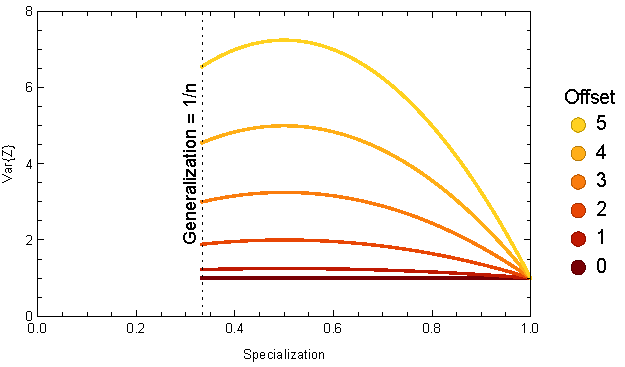
\includegraphics[width=0.5\textwidth]{fig_var.pdf}
\caption{
Variance of the isotopic distribution of diet with respect to specialization on a single prey, ${\rm Var}\{Z(s)\}$.
This illustrative example shows a three-prey system with prey means $\{-15,-15+\mbox{offset},-15\}$ and equal variances; colors depect specialization on prey 2 with a mean isotopic value that is a function of some offset amount.
As the offset of the targeted prey increases, so does the nonlinear nature of ${\rm Var}\{Z\}$.
}
  \label{figvar}
\end{figure}

\begin{figure}[h!]
\centering
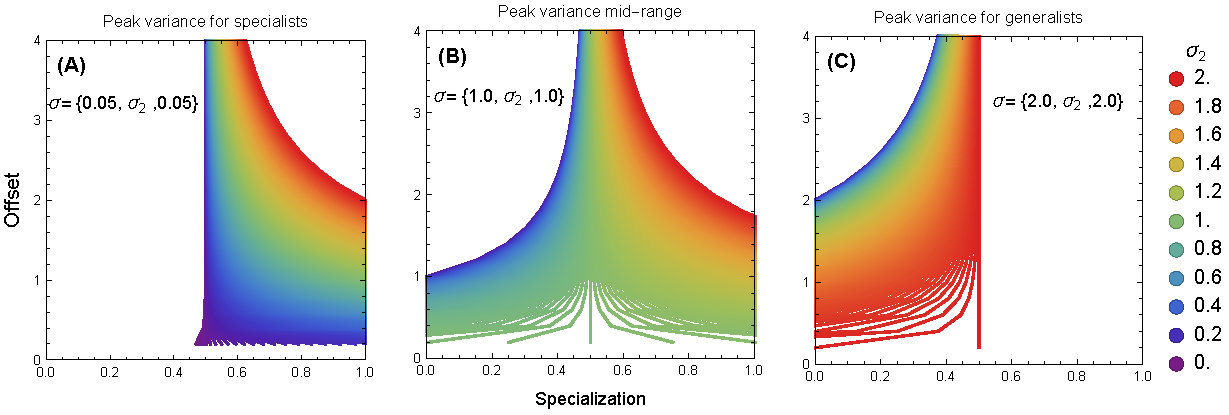
\includegraphics[width=1\textwidth]{fig_specvar.pdf}
\caption{
Maximal consumer isotopic varaince (niche width) over the specialization index $s$ as a function of mixing space geometry. A specialization value of $s=1/n$ denotes obligate generalization, while $s=1$ denotes obligate specialization.
Left, center, and right panel show the effect of different mixing space geometries on the location of maximal consumer niche width over $s$.
All panels: as the mean offset of the targeted prey is farther from the centroid of the mixing space, the maximal consumer isotopic niche width tends towards $s=0.5$.
Left and Center panel: If the targeted prey has a higher than average isotopic variance, the maximum consumer niche width will lie towards consumer specialization.
Center and Right panel: If the targeted prey has a lower than average isotopic variance, the maximum consumer niche width will like towards consumer generalization.
}
  \label{figspecvar}
\end{figure}



\begin{figure}[h!]
\centering
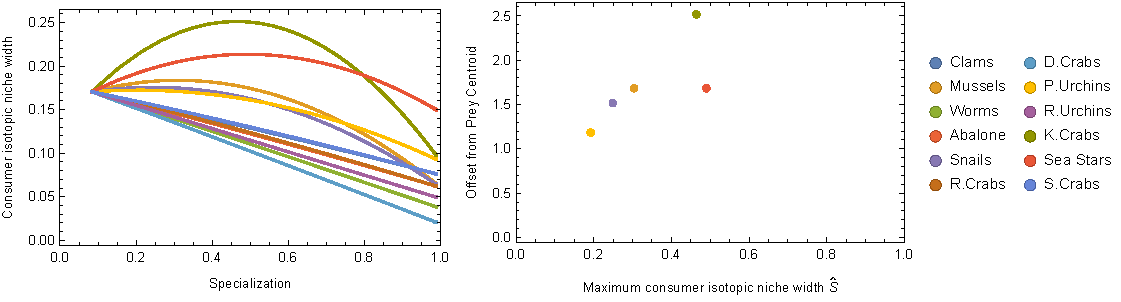
\includegraphics[width=1\textwidth]{fig_ottervar.pdf}
\caption{
Left panel: Predicted sea otter isotopic niche width over different degrees of specialization on each prey in the system (colors).
Right panel: Calculated maximum consumer niche width values as a function of specialization and the offset of the prey mean from the mixing space centroid.
}
  \label{figottervar}
\end{figure}

\begin{figure}[h!]
\centering
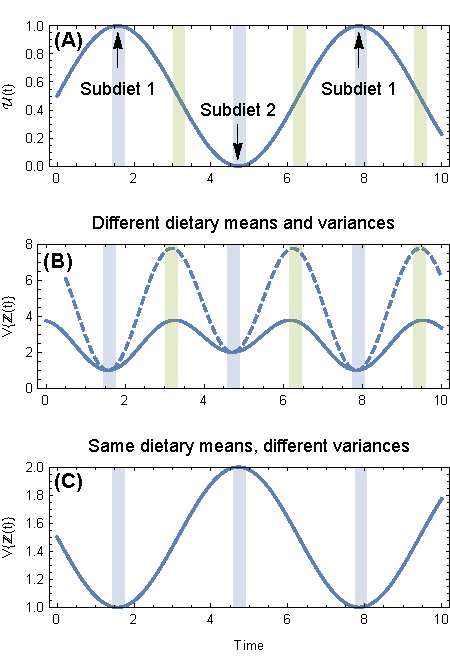
\includegraphics[width=0.4\textwidth]{fig_varZt.pdf}
\caption{
}
  \label{figvarZt}
\end{figure}

\begin{figure}[h!]
\centering
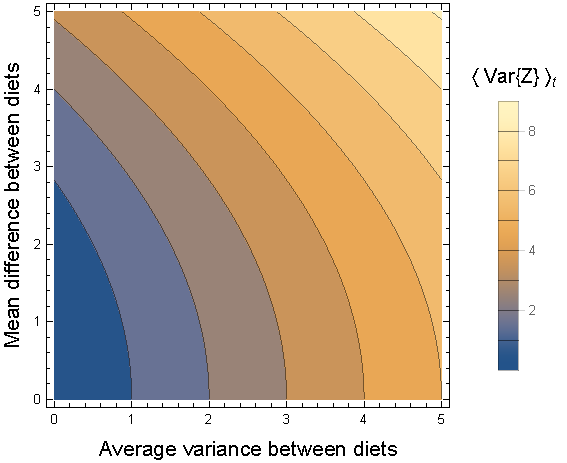
\includegraphics[width=0.4\textwidth]{fig_varzContour.pdf}
\caption{
}
  \label{figvarcont}
\end{figure}


\begin{figure}[h!]
\centering
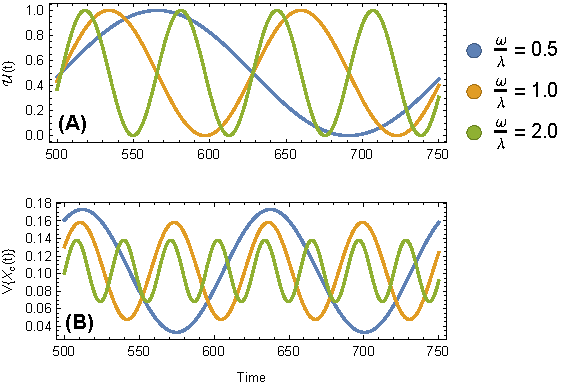
\includegraphics[width=0.5\textwidth]{fig_xcsin.pdf}
\caption{
}
  \label{figxcsin}
\end{figure}

\begin{figure}[h!]
\centering
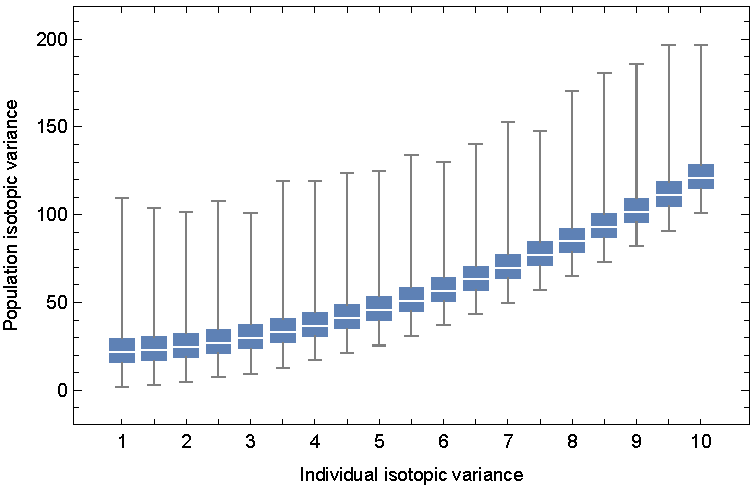
\includegraphics[width=0.5\textwidth]{fig_indpopvar.pdf}
\caption{
}
  \label{figindpopvar}
\end{figure}


\end{document}
